\subsection{Sensor Data Preprocessing}
\label{subsec:transformations}

Each radar sensor in the dual-radar configuration is physically mounted with a specific orientation and tilt relative to the vehicle's forward direction. 
To ensure a common frame of reference for all points, it is necessary to compensate for:

\begin{itemize}
    \item \textbf{Yaw rotation}: due to angled placement (±30$^\circ$) of the radar modules.
    \item \textbf{Pitch tilt}: due to upward mounting tilt (15$^\circ$), which must be compensated to recover horizontal geometry.
    \item \textbf{Sensor offset}: due to the physical separation of the radar sensors in the horizontal axis (X-axis).
\end{itemize}

A yaw rotation \( R_{\text{yaw}} \) was first implemented, followed by a pitch correction \( R_{\text{pitch}} \), and finally a translation vector \( \vec{t} \) was applied to account for the physical position of the sensors with respect to the vehicle's coordinate origin.

The full transformation can be expressed as:

\begin{equation}
T_{\text{veh}} = R_{\text{yaw}} \cdot R_{\text{pitch}} \cdot \vec{p}_{\text{radar}} + \vec{T}
\label{eq:radar_to_vehicle_transform}
\end{equation}

Where:
\begin{itemize}
    \item \( \vec{p}_{\text{radar}} \) is a radar point in sensor coordinates.
    \item \( R_{\text{yaw}} \) is a 2D rotation around the vertical axis.
    \item \( R_{\text{pitch}} \) corrects for the upward sensor tilt.
    \item \( \vec{T} \) is the translation vector.
\end{itemize}

\vspace{1em}

Let $(x, y, z)$ be the original point from the radar frame, with $x$ to the right, $y$ forward, and $z$ upward. 
The transformations applied are as follows:

\paragraph{Yaw Correction (Z-axis Rotation)}
The radar sensors are rotated relative to the vehicle frame:

\begin{itemize}
    \item Radar A (Left): Mounted at $+30^\circ$ yaw $\Rightarrow$ compensated with $-30^\circ$ rotation.
    \item Radar B (Right): Mounted at $-30^\circ$ yaw $\Rightarrow$ compensated with $+30^\circ$ rotation.
\end{itemize}

The 2D rotation in the XY-plane is defined as:
\[
\begin{bmatrix}
x' \\
y' \\
z'
\end{bmatrix}
=
\begin{bmatrix}
\cos(\theta) & -\sin(\theta) & 0 \\
\sin(\theta) & \cos(\theta) & 0 \\
0 & 0 & 1
\end{bmatrix}
\begin{bmatrix}
x \\
y \\
z
\end{bmatrix}
\]

where $\theta = \pm30^\circ$ depending on the sensor.

\begin{figure}[!htbp]
    \centering
    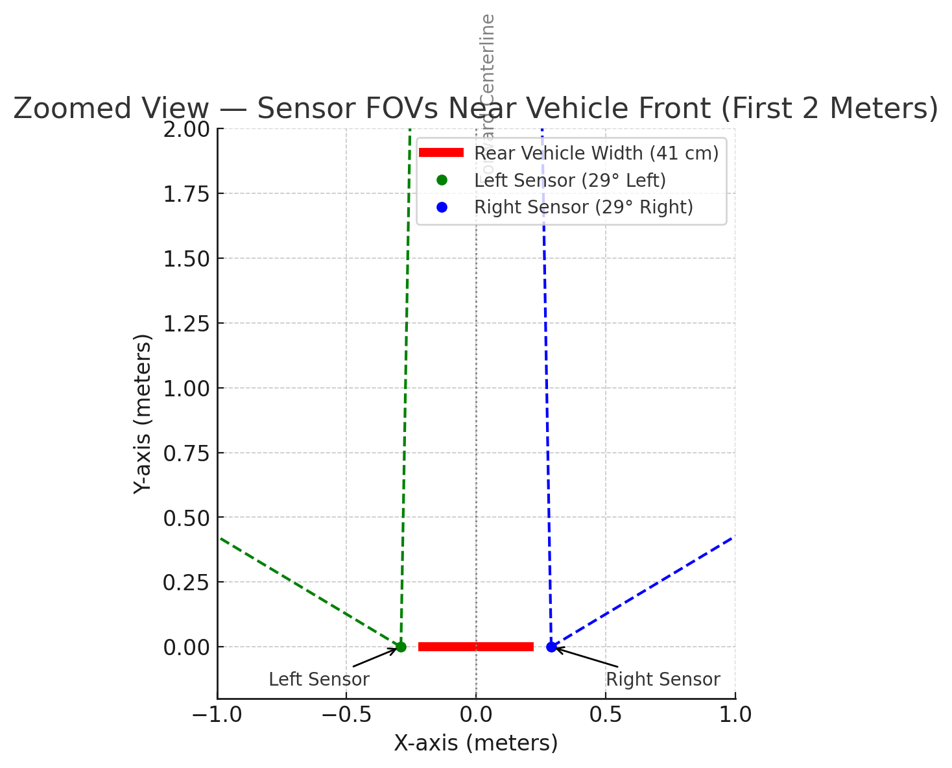
\includegraphics[width=0.8\linewidth]{images/SensorsRotation.png}
    \caption{Yaw rotation of sensors around the Z-axis (±30$^\circ$).}
    \label{fig:z_axis_rotation}
\end{figure}

\vspace{2em}

\paragraph{Pitch Compensation (X-axis Rotation)}
Since the radar sensors are tilted upward by $15^\circ$, a corrective rotation around the X-axis is applied to bring the points back to a horizontal perspective: 

\[
\begin{bmatrix}
x' \\ y' \\ z'
\end{bmatrix}
=
\begin{bmatrix}
1 & 0 & 0 \\
0 & \cos(\phi) & -\sin(\phi) \\
0 & \sin(\phi) & \cos(\phi)
\end{bmatrix}
\begin{bmatrix}
x \\ y \\ z
\end{bmatrix}
\]

where $\phi = -15^\circ$ (negative to reverse the upward tilt).

\begin{figure}[!htbp]
    \centering
    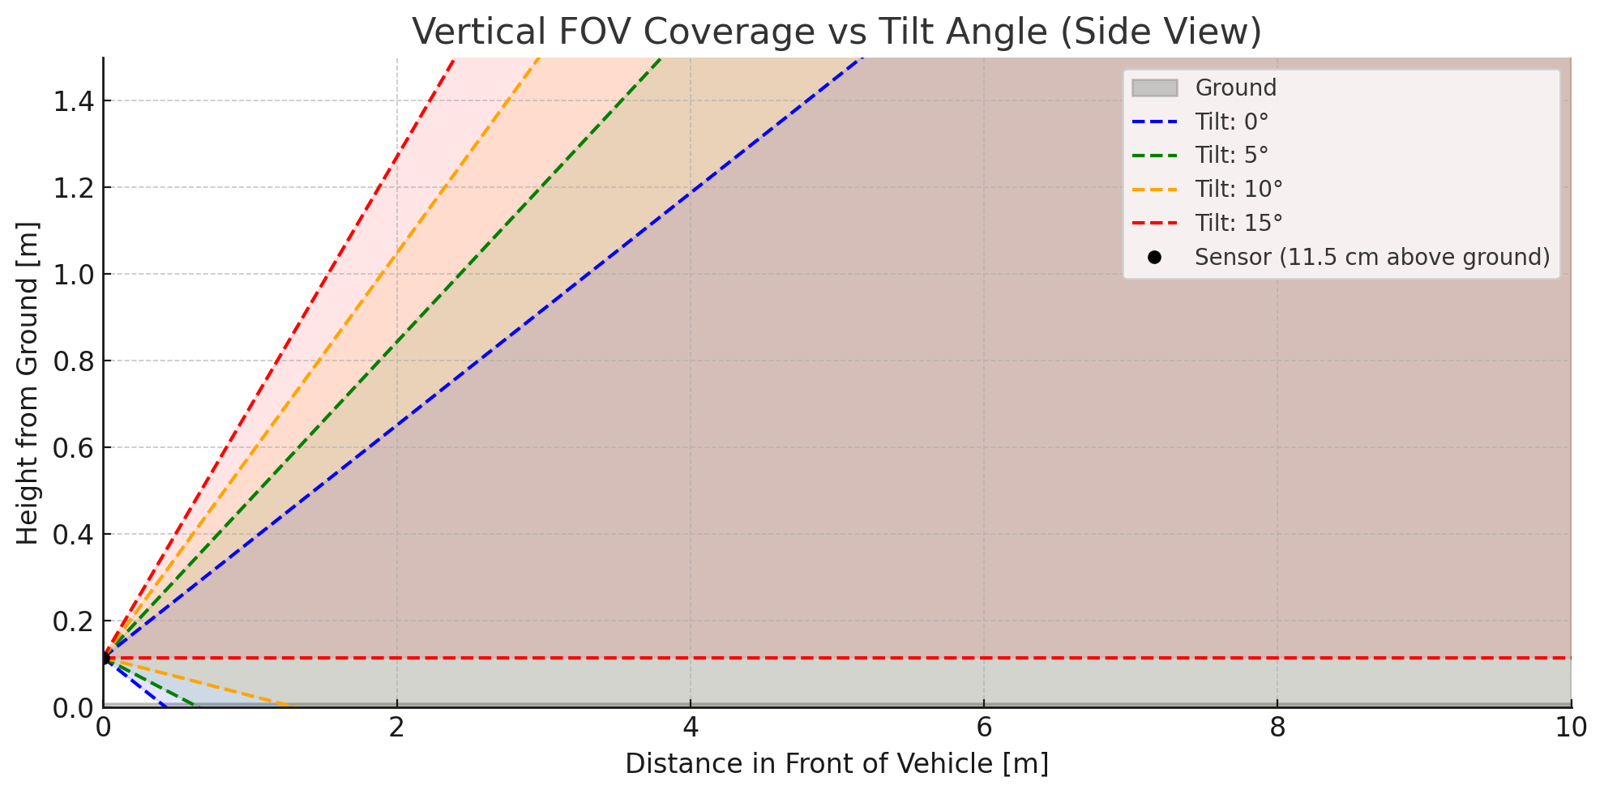
\includegraphics[width=0.8\linewidth]{images/TiltSensor.png}
    \caption{Pitch compensation for $15^\circ$ upward tilt.}
    \label{fig:x_axis_rotation}
\end{figure}

\vspace{2em}

\paragraph{X-Axis Offset Compensation}
After rotation, each sensor's point cloud was translated along the X-axis to align with the vehicle's center:
\begin{itemize}
    \item Radar A: $x \leftarrow x - 0.32$ meters
    \item Radar B: $x \leftarrow x - 0.28$ meters
\end{itemize}

This translation ensured both sensors were aligned in a common vehicle-centric frame.

\begin{figure}[!htbp]
    \centering
    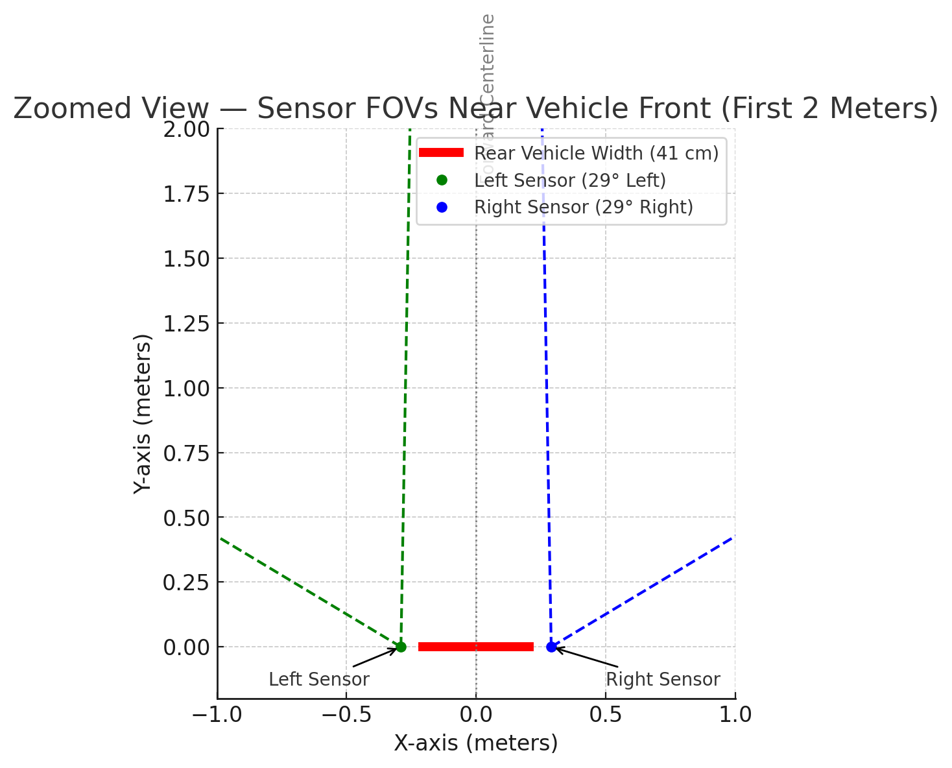
\includegraphics[width=0.8\linewidth]{images/RotationSensor.png}
    \caption{Final extrinsic configuration combining yaw, pitch, and translation.}
    \label{fig:extrinsics}
\end{figure}

\vspace{2em}

\paragraph{Impact of Transformations}
The importance of these corrections becomes evident when comparing raw and transformed data when the system data is unified in a single data set. 
Without transformations, detections from the left and right radars appear misaligned, producing duplicated or inconsistent clusters. 
After applying yaw, pitch, and translation compensation, the fused point cloud exhibits coherent structures, with static landmarks consistently overlapping across sensors.

Figures~\ref{fig:dualSensorCalib_2mts}--\ref{fig:AFTERdualSensorCalibRANSAC_2mts} illustrate this process, showing raw point clouds, clustered representations, and RANSAC fits before and after calibration. 
This information is of a person standing at 2 meters away form the vehicle, the process was decided as it was easy to visualize and to validate what was detected.
The transformed data serves as a stable basis for subsequent steps in the odometry pipeline, such as ICP-based submap alignment.

\begin{figure}[!htbp]
    \centering
    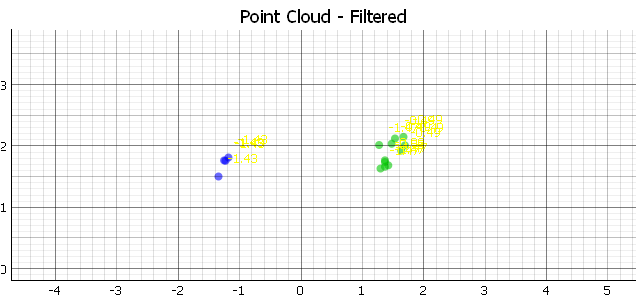
\includegraphics[width=0.9\linewidth]{images/dualSensorCalib_2mts.png}
    \caption{Raw dual-sensor point cloud before geometric transformations.}
    \label{fig:dualSensorCalib_2mts}
\end{figure}

\begin{figure}[!htbp]
    \centering
    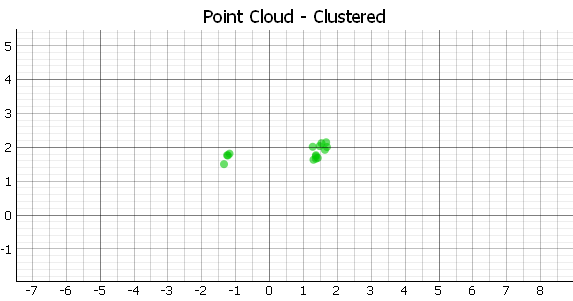
\includegraphics[width=0.9\linewidth]{images/dualSensorCalibCluster_2mts.png}
    \caption{Clustered detections from both radars before transformation.}
    \label{fig:dualSensorCalibCluster_2mts}
\end{figure}

\begin{figure}[!htbp]
    \centering
    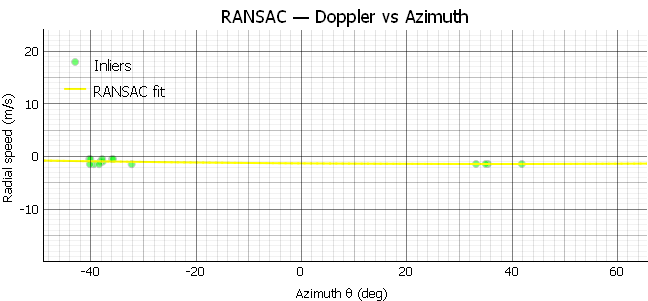
\includegraphics[width=0.9\linewidth]{images/dualSensorCalibRANSAC_2mts.png}
    \caption{RANSAC fit on Doppler velocities before transformation.}
    \label{fig:dualSensorCalibRANSAC_2mts}
\end{figure}

\begin{figure}[!htbp]
    \centering
    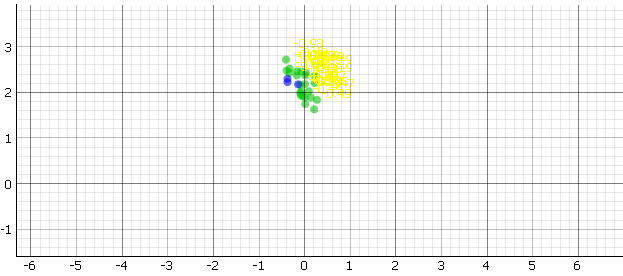
\includegraphics[width=0.9\linewidth]{images/AFTERdualSensorCalib_2mts.png}
    \caption{Fused point cloud after geometric transformations.}
    \label{fig:AFTERdualSensorCalib_2mts}
\end{figure}

\begin{figure}[!htbp]
    \centering
    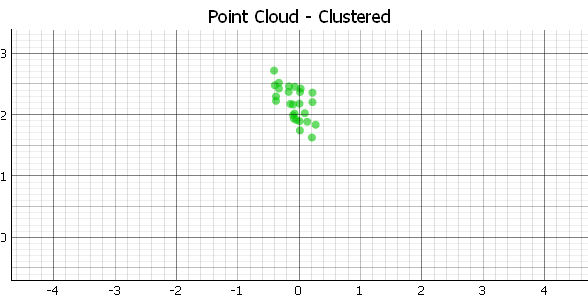
\includegraphics[width=0.9\linewidth]{images/AFTERdualSensorCalibCluster_2mts.png}
    \caption{Clustered detections after transformation, showing improved alignment.}
    \label{fig:AFTERdualSensorCalibCluster_2mts}
\end{figure}

\begin{figure}[!htbp]
    \centering
    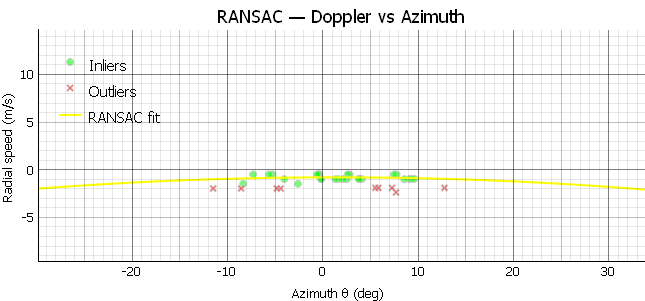
\includegraphics[width=0.9\linewidth]{images/AFTERdualSensorCalibRANSAC_2mts.png}
    \caption{RANSAC fit on Doppler velocities after transformation.}
    \label{fig:AFTERdualSensorCalibRANSAC_2mts}
\end{figure}

\vspace{1em}

\paragraph{Summary of Extrinsics}
\begin{itemize}
    \item \textbf{Left radar:} yaw $+30^\circ$, pitch $-15^\circ$, translation $(-0.32, 0, 0)$.
    \item \textbf{Right radar:} yaw $-30^\circ$, pitch $-15^\circ$, translation $(-0.28, 0, 0)$.
\end{itemize}

This extrinsic calibration ensures that dual-radar data is expressed in a coherent vehicle-centric frame, which is critical for downstream modules such as clustering, odometry, and obstacle tracking.
